\section{Azioni globali}
In questa sezione verranno descritte tutte le azioni che possono essere svolte generalmente, senza quindi dover accedere a modalità
di progettazione particolare.

	\subsection{Menù File}
		\begin{figure}[H]
			\centering
				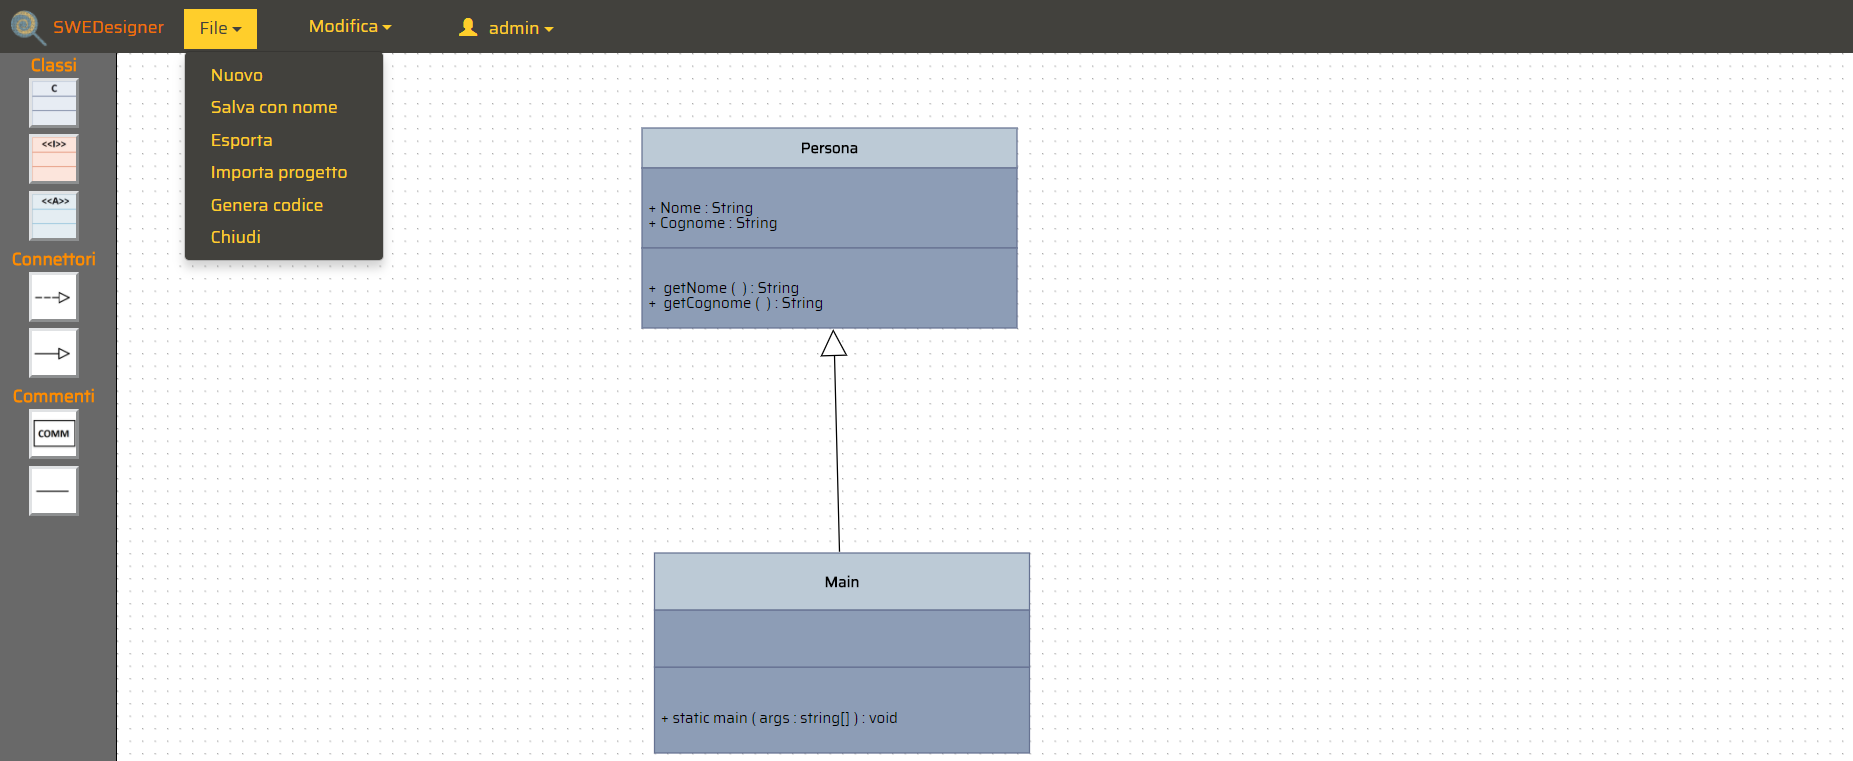
\includegraphics[width=1\linewidth]{res/img/menuFile.png}
			\caption{Menù File}
		\end{figure}
		Il menù \emph{File} consente di effettuare tutte le operazioni di salvataggio, esportazione e importazione del progetto.\\
		È possibile, inoltre, aprire un nuvoo progetto e generare il codice del progetto corrente oltre a chiude l'applicazione.\\
		\subsubsection{Nuovo progetto}
			Per creare un nuovo progetto selezionare, all'interno della voce \emph{File}, \emph{Nuovo}.
			Tale operazione ricaricherà l'editor completamente vuoto.
		\subsubsection{Salvataggio progetto}

			\begin{figure}[H]
				\centering
					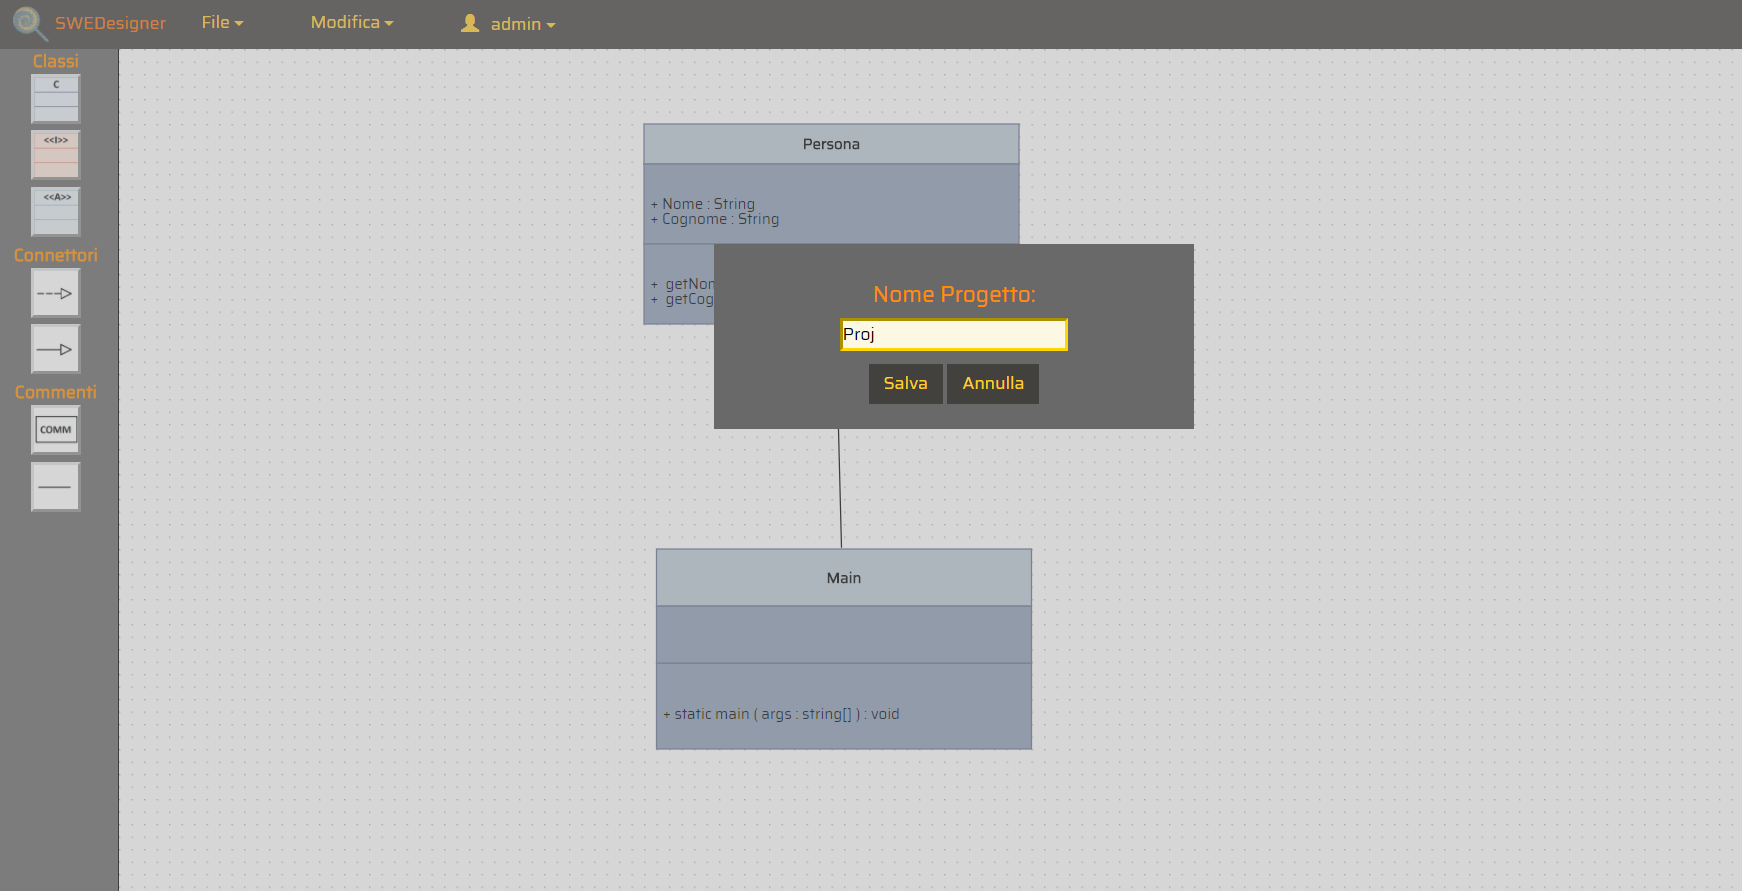
\includegraphics[width=1\linewidth]{res/img/salvaConNome.png}
				\caption{Esportazione progetto}
			\end{figure}

			Per salvare il progetto corrente all'interno del database selezionare, all'interno della voce \emph{File}, \emph{Salva con nome}.
			Verrà visualizzato un pop-up in cui verà richiesto il nome del progetto.\\
			Premendo sul tasto \emph{Annulla} si ritornerà indietro all'editor, mentre, selezionando \emph{Salva} verrà salvato il progetto all'interno del database.
		\subsubsection{Esportazione progetto}
			Per esportare il progetto in uso su un file locale, dal menu superiore, all'interno della voce \textit{File} selezionare \textit{Esporta}.\\
			Verrà scaricato nella vostra directory predefinita di download un file \emph{.json} contente il progetto crittografato.\\
		\subsubsection{Importazione progetto}
			Per importare un progetto è necessario fare un click su \textit{File} e, di seguito, su \emph{Importa}.\\
			Verrà visualizzata una finestra di esplorazione del filesystem dalla quale bisogna selezionare il file \emph{.json} del progetto da importare.\\
			Qualora il file non fosse valido non verrà visualizzato nulla sull'editor.\\
		\subsubsection{Generazione codice}
			Per generare il codice dal progetto corrente è necessario fare un click su \textit{File} e, di seguito, su \emph{Genera codice}.\\
			Verrà scaricato nella vostra directory predefinita di download un file \emph{.zip} contente il programma Java compilato e pronto all'esecuzione.\\
			È assolutamente necessario che la classe principale, contentente il Main, deve essere rinominata in Main.\\
	\subsection{Menù modifica}
		\begin{figure}[H]
			\centering
				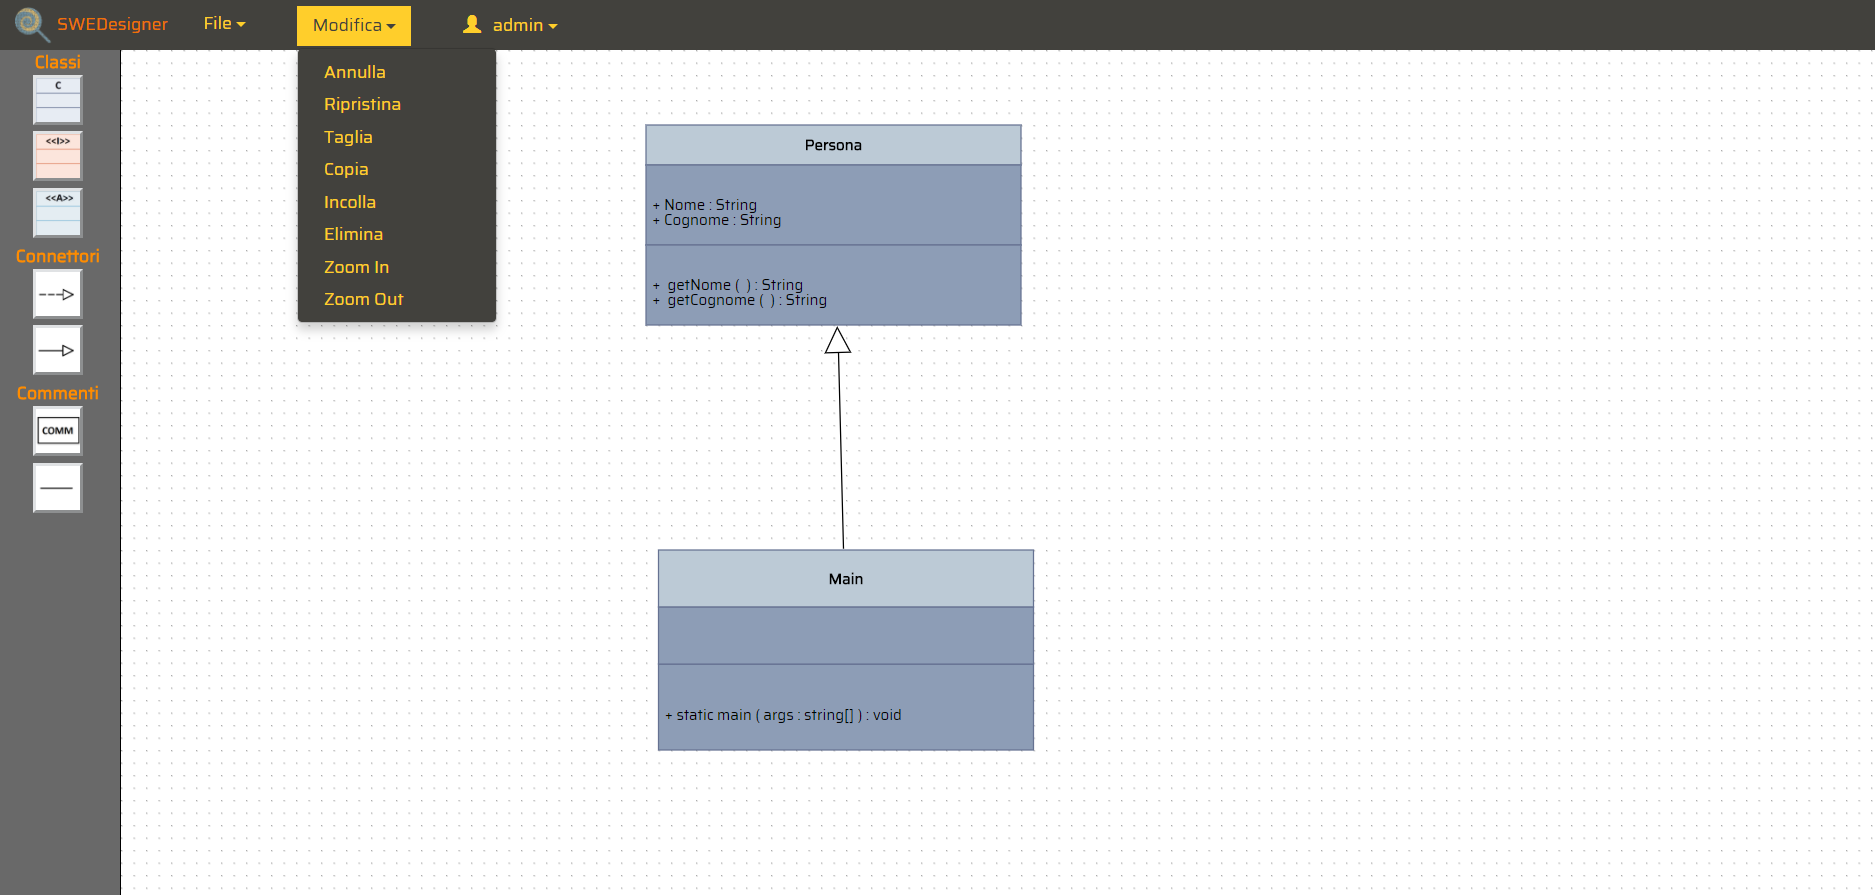
\includegraphics[width=1\linewidth]{res/img/menuModifica.png}
			\caption{Menù Modifica}
		\end{figure}
		All'interno di questa sezione del menù è possibile effettuare le classiche operazioni di modifica all'interno del progetto corrente.\\
		Si può effettuare, tramite il click su ognuna delle voci, un'operazione di \emph{Taglia}, \emph{Copia}, \emph{Incolla}, \emph{Annulla}, \emph{Ripristina}, \emph{ZoomIn} e \emph{ZoomOut}.\\
		Per ognuna di queste operazioni è necessario selezionare un elemento all'interno dell'editor.\\
	\subsection{Menù profilo}
		\begin{figure}[H]
			\centering
				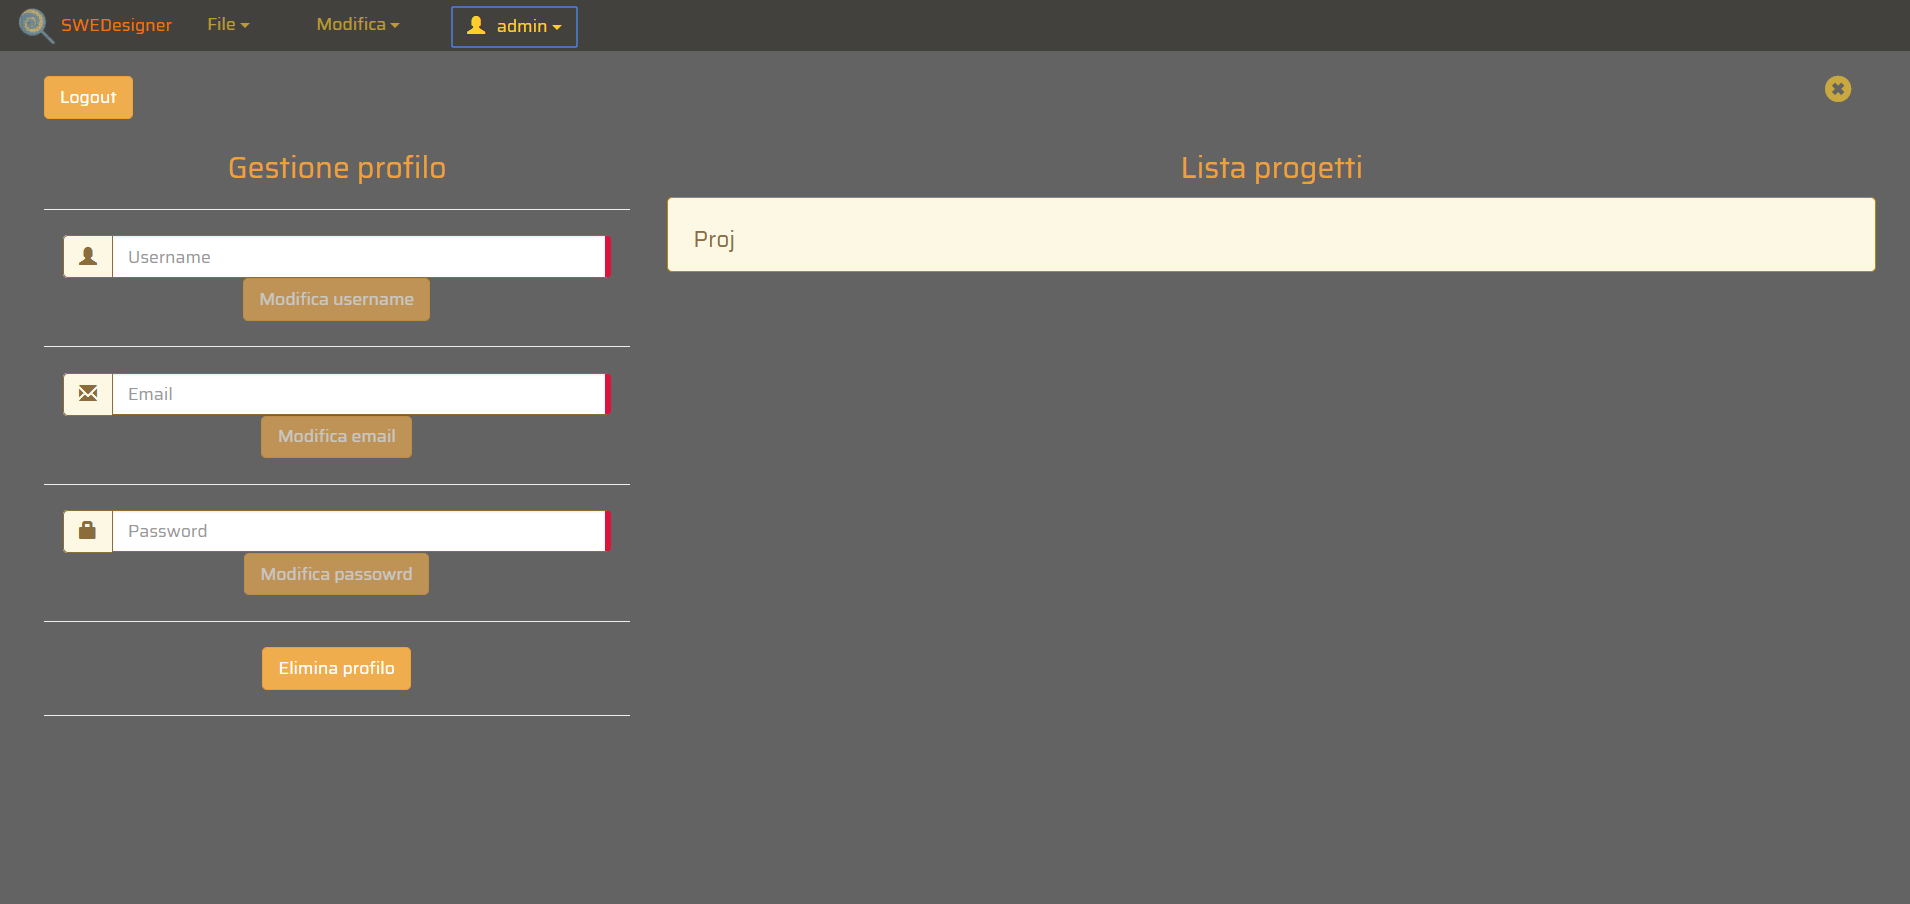
\includegraphics[width=1\linewidth]{res/img/menuProfilo.png}
			\caption{Menù Proilo}
		\end{figure}
		All'interno di questo menù è possibile gestire tutto ciò che riguarda l'utente e gestire i progetti salvati sul database.
		\subsubsection{Gestione profilo}
			In questa sezione  è possibile modificare singolarmente:
			\begin{itemize}
				\item Username
				Con l'inserimento del nuovo username nell'apposito campo seguito da un click sul tasto \emph{Modifica Username}
				\item Password
				Con l'inserimento della nuova password nell'apposito campo seguito da un click sul tasto \emph{Modifica Password}
				\item E-Mail
				Con l'inserimento della nuova e-mail nell'apposito campo seguito da un click sul tasto \emph{Modifica email}
			\end{itemize}
			In questa sezione è possibile, inoltre, eliminare il proprio profilo mediante un click sul tasto \emph{Elimina profilo} seguito
			da un click sul bottone \emph{Sì} qualora si fosse sicuri o \emph{No} se si volesse tornare indietro.\\
			Infine, con un click su \emph{Logout} è possibile ritornare alla pagina di autenticazione.
		\subsubsection{Lista progetti}
			In questa sezione è possibile visualizzare la lista dei propri progetti.\\
			Selezionadoli con il mouse è possibile visualizzare l'icona di un cestino o quella di una cartalla che, rispettivamente, elimina o apre un progetto.

	\subsection{Designer classi}
		In questa sezione sarà descritto il comportamento dell'editor delle classi, quindi il loro disegno e i collegamenti fra di esse.\\
		Ognuno degli strumenti descritti si trova nella barra a sinistra dell'editor.\\
		\subsubsection{Classi}
			In questa sezione  è possibile utilizzare gli strumenti per il disegno di una \emph{Classe}, \emph{Interfaccia} o \emph{Classe astratta}.\\
			Mediante il click sui singoli bottoni la classe verrà disegnata nell'angolo in alto a sinistra e potrà essere spostata a piacimento all'interno dell'editor.\\
			La personalizzazione di tali classi sarà descritta nel capitolo successivo.
		\subsubsection{Connettori}
			In questa sezione è possibile connettere le classi fra di loro creando delle relazioni.\\
			Sono disponibili sia il connettore per le \emph{Interfaccie} e \emph{Classi astratte} sia quello per le classi normali.\\
			Per connettere un elemento ad un altro basta selezionare il connettore desiderato, fare un click sulla classe di arrivo e uno su quella di partenza.\\
		\subsubsection{Commenti}
			\begin{figure}[H]
				\centering
					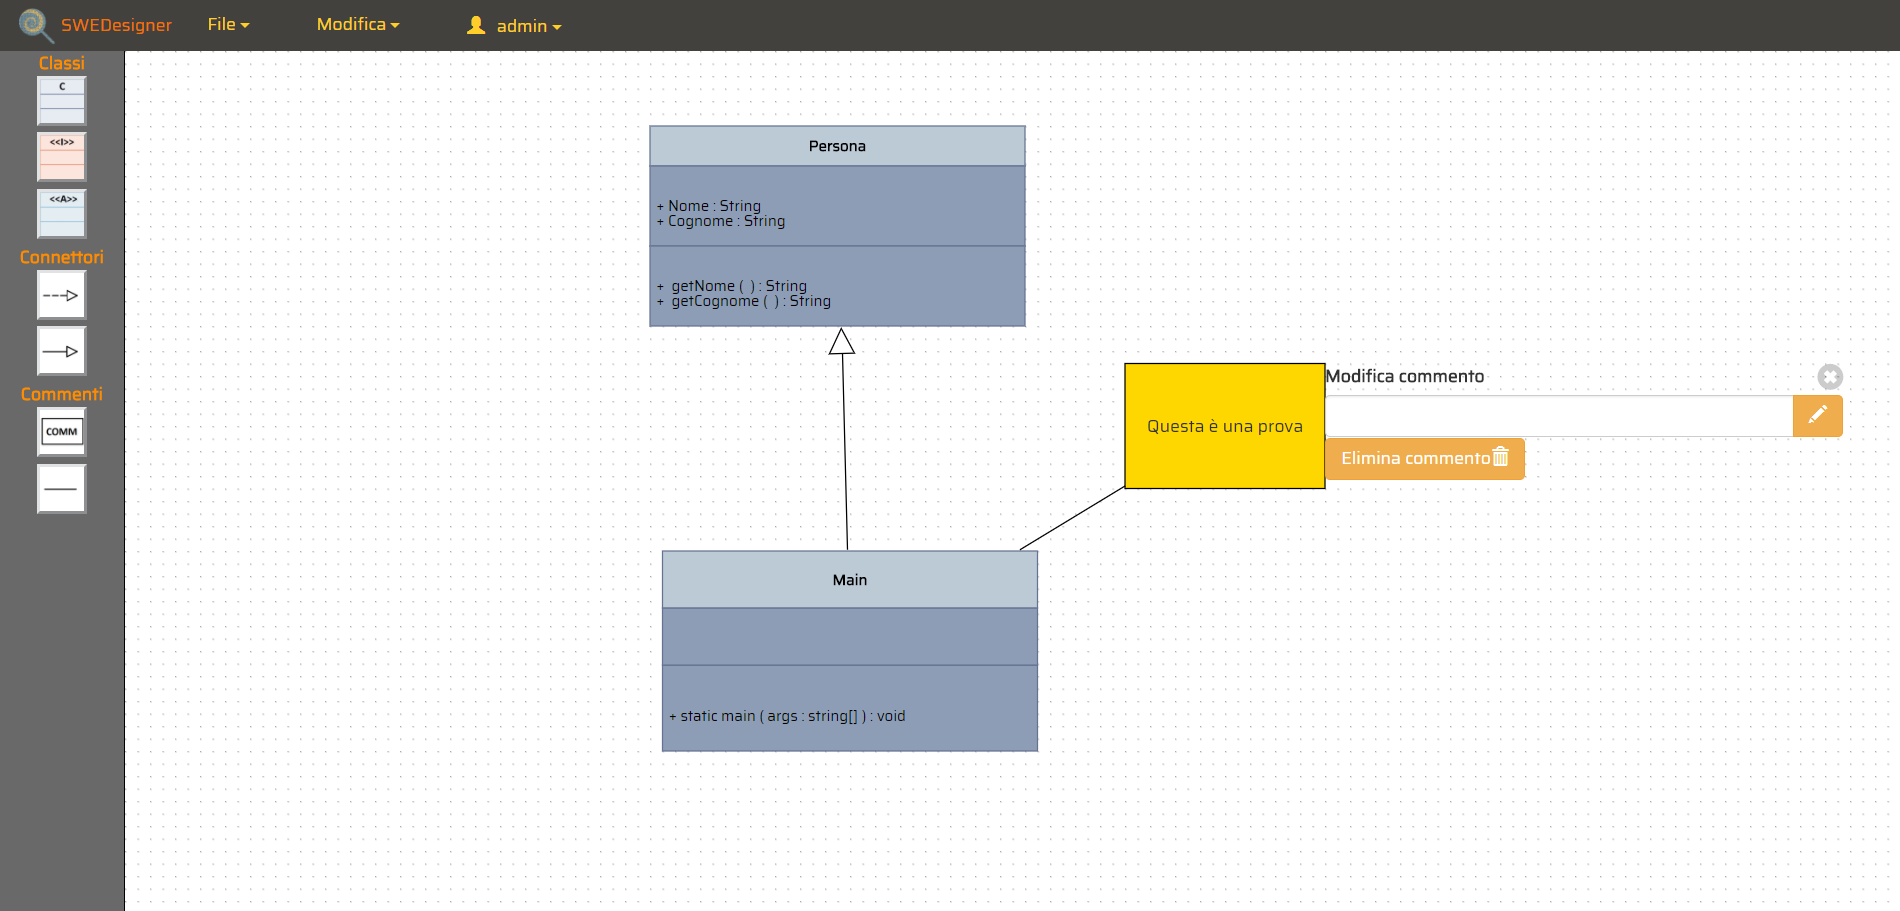
\includegraphics[width=1\linewidth]{res/img/designer1.png}
				\caption{Gestione commenti}
			\end{figure}
			In questa sezione  è possibile creare dei \emph{Commenti} e associarli ad una \emph{Classe}.\\
			Per creare un commento basterà fare un click sull'apposito bottone mentre, per aprire l'editor dello stesso, sarà richiesto un doppio click sul commento appena creato.\\
			Per connettere un commento ad una classe basterà fare un click sull'apposito bottone, fare un click sul commento e poi uno sulla classe a cui si vole assoociarlo.\\
